\documentclass{supervision}
\usepackage{course}

\Supervision{3}

% Could you do questions 7-10 inclusive for next week (as long as you have got
% that far in the lectures of course). You may find some of the terminology in
% parts of Q7 confusing/hard to find info on. If you do then skip those parts.

% I also am not certain if your course still covers suitable material to let
% you do all of Q9. Let me know if you think you can’t do it. Q10 also often
% causes students to struggle. I can recommend the wikipedia article on CRC
% codes

\begin{document}
  \begin{questions}
    %%%%%%%%%%%%%%%%%%%%%%%%%%%%%%%%%%%%%%%%%%
    \section*{Topic 03 - Data-Link (Physical)}
    %%%%%%%%%%%%%%%%%%%%%%%%%%%%%%%%%%%%%%%%%%
    \SetQuestionNumber{7}
    \question \textit{Shared media multiplexing in local area networks}
      \begin{parts}
        \part Define the term \textit{shared media network}
          \begin{solution}
            A shared media network is one where the bandwidth of a single
            medium is shared between all the nodes. Ethernet, Token ring and
            FDDI are examples of shared media networks.
          \end{solution}

        \part Explain how Ethernet performs \textit{carrier sense},
          \textit{collision detection}, how it aims to minimise the
          probability of collision on retransmission and how this is adapted
          to handle varying load.
          \begin{solution}
            The node first listens on the wire, if a transmission is already
            happening then it waits for it to finish (including the additional
            96 bit interframe gap period). The node then transmits the frame.

            If a collision occurs (the transmission gets trampled by another
            node that did carrier sense at almost the exact same time) then
            continue transmission with a jam signal until the minimum packet
            time is reached to ensure that all receivers detect the collision.
            After this, increment the retransmission counter - if it has
            reached the maximum number of attempts then abort transmision
            otherwise wait the backoff period (a random time period that
            exponentially grows with subsequent collisions).
          \end{solution}

        \part Explain why token ring does not share media at the physical
          level, but is still analyzed as a shared media system.
          \begin{solution}
            A token ring network consists of several unidirectional, point to
            point links joining the nodes in a ring. Each node therefore has
            its own physical link that is not shared with any other node. It is
            analyzed as a shared media system as for a frame to get to its
            destination it has to travel across multiple links, each of which
            is exclusively reserved for the token holder.
          \end{solution}

        \part What is the role of a token monitor in token ring? Why does the
          monitor \textit{not} prevent failure when one of the nodes in the
          ring suffers a hardware failure? Suggest how a token ring system
          might be designed to handle failure of a computer attached to the
          ring.
          \begin{solution}
            The token monitor ensures that tokens do not cycle around the ring
            endlessly. It does this by setting a monitor flag on the token as
            it passes and then if a token with the monitor flag set reaches it
            again it terminates it.

            To handle failure of a single node the ring could bounce tokens
            off of the end (treating the broken ring as a line).
          \end{solution}

        \part Explain the meaning of \textit{destination delete} and
          \textit{source delete} as used in ring-based networks.
          \begin{solution}
            \begin{description}
              \item[destination delete] Destination delete is where the
                destination node for a certain frame is responsible for
                rleasing the token.
              \item[source delete] Source delete is where the node where a
                frame originated is responsible for releasing the token.
            \end{description}
          \end{solution}

        \part Explain the difference between conventional token rings and
          \textit{slotted rings}. What are the advantages of a slotted ring?
          \begin{solution}
            A slotted ring is divided into fixed size slots, each with a bit
            which can be set to full or empty. The advantage is that higher
            throughput can be achieved? \emph{Not sure about this - finding it
            hard to find relevant information}
          \end{solution}
      \end{parts}

    \question \textit{Multiplexing redux}
      \begin{parts}
        \part Several real-time video streams are to share the same
          lower-layer channel.
          \begin{subparts}
            \subpart Give one example of a lower-layer channel in which the
              flows might be scheduled, and one in which scheduling is not
              possible.
              \begin{solution}
                \begin{description}
                  \item[Streaming Netflix] Can use scheduling
                  \item[Terrestrial TV] Uses FDMA and therefore scheduling is
                    not possible.
                \end{description}
              \end{solution}


            \subpart A lecturer remarks that “centralised multiplexing”
              offers potential gains in efficiency over non-centralised
              multiplexing. Give two reasons why this can improve efficiency.
              What, in general terms, is the “centralised” facility necessary
              for these gains to be possible?
              \begin{solution}
                Without centralised multiplexing then collisions will occur
                leading to reduced transmission rates.

                With centralised multiplexing the multiplexer knows the length
                of all the queues and can make a decision about which packet to
                send next based upon various QoS objectives.

                Advanced multiplexers might might even perform introspection on
                the packets and prioritise certain packets (e.g. those
                belonging to a video stream/multiplayer game) over others (file
                downloads) which may give the illusion of a smoother running
                network as a user who is downloading a large file will not miss
                $5\%$ of their bandwidth but a user who is streaming video at
                $95\%$ of the bandwidth required for seemless playback will
                be very grateful for it.
              \end{solution}

            \subpart Using an example, describe why specifying a scheduling
              policy in terms of priority may cause problems, even where it
              is safe to use priority within the scheduling mechanism.
              [Hint: consider CPU scheduling in an operating system.]
              \begin{solution}
                Care has to be taken to ensure that the low-priority packets
                still make progress, it is counter productive to leave a packet
                in a queue for so long that the sender has assumed it was lost
                and resent it.
              \end{solution}
          \end{subparts}

        \part Code-division multiple access (CDMA) is a code-division
          multiplexing system, used for mobile telephony.
          \begin{subparts}
            \subpart What is a code? What property of codes causes them to be
              “nearly orthogonal” to each other?
              \begin{solution}
                \begin{description}
                  \item[Truly orthogonal codes] Two codes are said to be
                    orthogonal if when they are multiplied together, the sum
                    over a period of time is zero. An example of an
                    orthogonal code set is the Walsh codes.

                  \item[Pseudo noise codes] Another code type for CDMA is a
                    pseudo-random code, these can be generated very easily and
                    are used in mobile telephony as the handset to base-station
                    links cannot be coordinated due to the large quantity and
                    mobility of the handsets.

                    A PN code is a binary sequence that appears random but can
                    be reproduced in a deterministic manner by intended
                    receivers.

                    The Pseudo-random generators produce sequences that
                    when time shifted are nearly orthogonal (narrow ambiguity
                    function).
                \end{description}
              \end{solution}

            \subpart Two transmitters, A and B, both want to transmit a
              four-bit message at the same time using CDMA. Transmitter A has
              code 10010111 and message 1001. Transmitter B has code 00111101
              and message 0011. Write down the bit sequences transmitted by A
              and B. Write down the bit sequence seen by a receiver, stating
              any assumption you make. Show that the original messages of
              both A and B may be recovered. [Each bit is transmitted as the
              exclusive OR of the code sequence with the bit value.]
              \begin{solution}
                \begin{code}{{}}
                The bit sequence from A is encoded as:
                 1 -1 -1  1 -1  1  1  1
                -1  1  1 -1  1 -1 -1 -1
                -1  1  1 -1  1 -1 -1 -1
                 1 -1 -1  1 -1  1  1  1

                The bit sequence from B is encoded as:
                 1  1 -1 -1 -1 -1  1 -1
                 1  1 -1 -1 -1 -1  1 -1
                -1 -1  1  1  1  1 -1  1
                -1 -1  1  1  1  1 -1  1

                The signal seen by the receiver is:
                 2  0 -2  0 -2  0  2  0
                 0  2  0 -2  0 -2  0 -2
                -2  0  2  0  2  0 -2  0
                 0 -2  0  2  0  2  0  2

                The signal after combining with A's code:
                 2  0  2  0  2  0  2  0
                 0 -2  0 -2  0 -2  0 -2
                -2  0 -2  0 -2  0 -2  0
                 0  2  0  2  0  2  0  2

                And then after converting into message:
                1 0 0 1

                The signal after combining with B's code:
                -2  0 -2  0 -2  0 -2  0
                 0 -2  0 -2  0 -2  0 -2
                 2  0  2  0  2  0  2  0
                 0  2  0  2  0  2  0  2

                And then after converting into message:
                0 0 1 1
                \end{code}
              \end{solution}
          \end{subparts}
      \end{parts}

    \question \textit{Coding, digitisation, error detection and error
      correction}
      \begin{parts}
        \part Give, with examples, three advantages of digitising audio, and
          three corresponding disadvantages. (Compare with storing and
          processing it exclusively on analogue media and equipment.)
          \begin{solution}
            Different types of audio have different characteristics, speech
            is typically within the range \SIrange{300}{3400}{\Hz} whilst music
            contains many repeating waves. These properties make them ideal for
            digitisation as they can be heavily compresses without losing any
            perceivable quality. In the first case the other frequencies can be
            safely ``chopped off'' and in the second the audio can be
            represented using a fourier transform. This gives the advantage
            that less space is required to store it.
          \end{solution}

        \part Explain quantisation and sampling of analogue signals, and the
          distinction between these. State an upper bound for the
          signal-to-noise ratio of a signal quantised at $b$ bits resolution,
          assuming the analogue original to be noiseless and the quantisation
          process completely accurate.
          \begin{solution}
            \emph{Skipped as per email}
          \end{solution}

        \part Outline encode and decode procedures for a simple ($m$,$k$)
          block code. Show that the minimum distance of any simple checksum
          code is always $2$.
          \begin{solution}
            \emph{Skipped as per email}
          \end{solution}

      \end{parts}

    \SetQuestionNumber{10}
    \question \textit{CRCs}
      \begin{parts}
        \part Explain, giving an example, how to write a binary message (i.e.
          a sequence of binary digits) as a polynomial.
          \begin{solution}
            Each bit is a coefficient of terms in increasing order of power.

            E.g. $010111$ becomes $0x^5 + 1x^4 + 0x^3 + 1x^2 + 1x + 1$ which
            simplified is $x^4 + x^2 + x + 1$.
          \end{solution}

        \part Outline send and receive procedures for CRC-based message
          coding and error detection. What information must be agreed in
          advance by the sender and reciever?
          \begin{solution}
            To send a message $M(x)$ of size $k$ bits. We find the remainder:
            \begin{equation*}
              R(x) = x^n M(x) \: {rem} \: P(x)
            \end{equation*}
            and send:
            \begin{equation*}
              T(x) = x^n M(x) \: {rem} \: P(x)
            \end{equation*}
          \end{solution}

        \part Draw a shift register which will compute the remainder on
          division of an input polynomial by the CRC-8 polynomial
          $x^8 + x^2 + x^1 +1$.
          \begin{solution}
            \begin{center}
              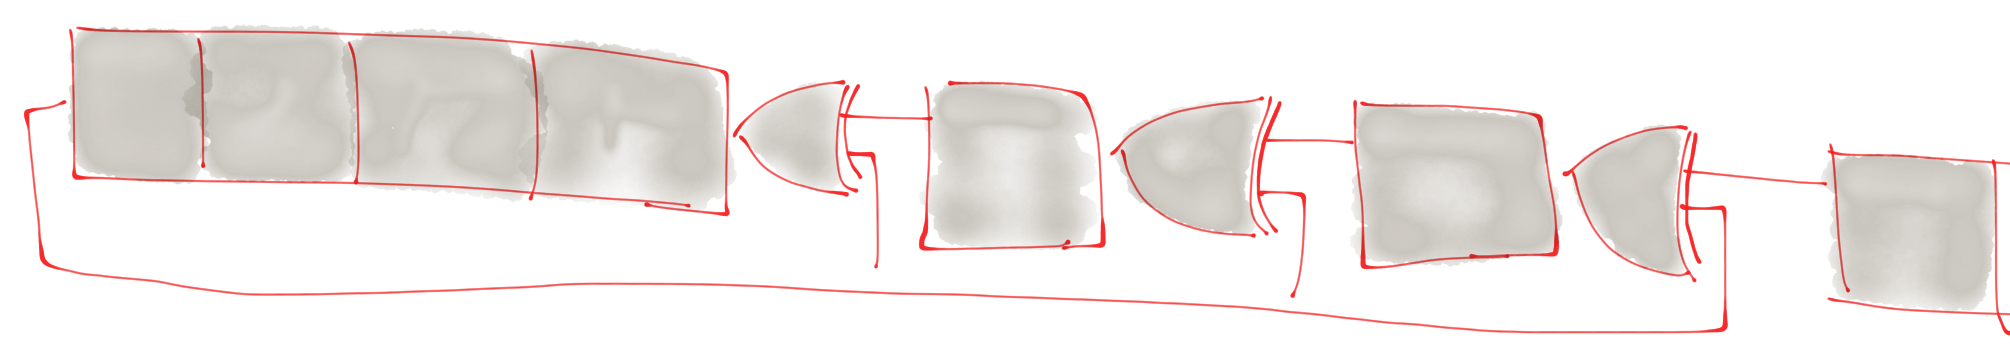
\includegraphics[width=0.9\textwidth]{10-crc-shift-register}
            \end{center}
          \end{solution}

      \end{parts}
  \end{questions}
\end{document}
